\chapter{Credit Risk Modelling}
\label{chap:two}


\section{Formal requirements of master's thesis}
\label{sec:formal}

According to \href{https://www.fsv.cuni.cz/deans-provision-no-182017}{Dean's Provision no.\ 18/2017}:
\begin{itemize}
		\item  The minimum extent of master's thesis is 60 standard pages (108 thousand characters including spaces) of the text itself, i.e. without an abstract and appendices and a list of literature. In case the master's thesis is written in English, its minimum extent is 50 standard pages (90 thousand characters including spaces) without an abstract and appendices and a list of literature. When writing a standard text document, the minimum requirement is 60 characters per line and 30 lines per page, i.e. 1,800 characters per page (the so-called standard page). Font size, page layout, margins, and line spacing need to be customized.
		\item Generally, a standard form of the page of the final thesis applies the fonts of 12 points, the gaps between the paragraphs are recommended to be of the size of 6 points. Notes and footnotes can be written in a 10-point font. The text is aligned on both sides (aligned to a block). Electronic version of the thesis will be entered by a student/applicant for a state examination through the SIS website interface in the archive format of PDF/A version 1.3 or higher. Further details are stipulated by the rector's provision.
		\item The master's thesis is submitted in the accreditation language of the respective follow-up Master's study program. 
\end{itemize}

Note that due to GDPR, the thesis cannot include any personal information (phone, e-mail) or signatures (neither of the author nor of the supervisor).

\section{Template adjustments and meta-data}
\label{sec:metadata}

Read README.txt to get a jist of how the template works and how to adjust styles. You can change the properties of your pdf file, such as title, author, keywords, or publisher

\begin{figure}[!h]
	\centering
		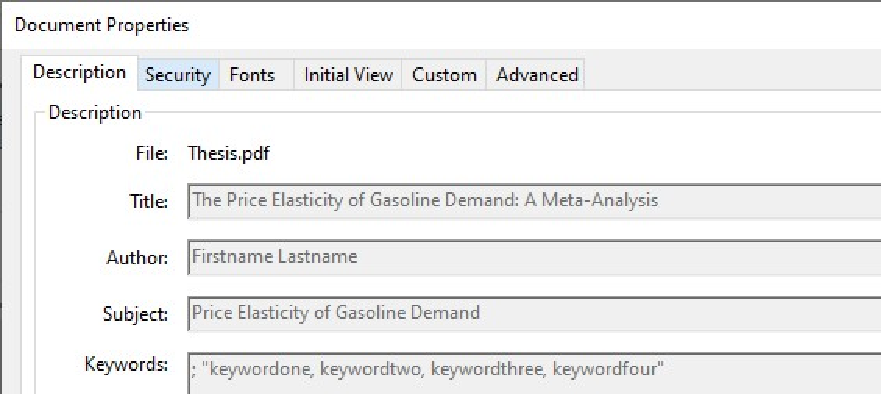
\includegraphics[width=0.96\textwidth]{Figures/properties.pdf}
	\label{fig:properties}
\end{figure}

\noindent in \textbf{Thesis.xmpdata} file. The file is editable in any text editor.



